Se implementó un modelo de clasificación con el propósito de predecir y comprender el comportamiento del usuario basándose en un conjunto de datos detallado y complejo.

\subsection{Preprocesamiento y Preparación de Datos}

Comenzamos con la importación de los datos desde un archivo CSV, seguida de un proceso de limpieza para asegurar la integridad de la información. En esta etapa, se filtraron registros específicos en la columna “método” y se descartaron aquellos casos donde la columna “canal” estaba vacía. Adicionalmente, las marcas temporales fueron convertidas al formato UTC para garantizar una estandarización completa a lo largo del conjunto de datos.

El preprocesamiento es un paso fundamental para asegurarse de que los datos estén limpios, relevantes y listos para el modelado. Durante esta fase, se eliminan o corrigen valores atípicos, se manejan valores faltantes y se asegura la consistencia de los datos. Se filtraron métodos específicos y se eliminaron registros donde el canal estaba vacío para mantener solo los datos que contribuyen significativamente al análisis. La conversión de marcas temporales a UTC garantiza que todas las fechas y horas estén en un marco de referencia uniforme, lo cual es crítico para análisis temporales y comparaciones de eventos a través de diferentes zonas horarias.

\subsection{Ordenamiento y Etiquetado}

Para preservar la secuencia de acciones de cada usuario, ordenamos el conjunto de datos cronológicamente por usuario y fecha de evento. Este ordenamiento cronológico es esencial para cualquier modelo de clasificación secuencial, ya que permite comprender y aprender de las transiciones entre diferentes acciones o estados de un usuario. Específicamente, agrupamos las acciones por la columna \textquotedblleft rut\_cliente\textquotedblright y, dentro de cada grupo, las ordenamos por \textquotedblleft fecha\_evento\textquotedblright para mantener la secuencia temporal de las actividades.

Tras el ordenamiento, procedimos con la generación de etiquetas para la supervisión del aprendizaje. Excluyendo la última acción de cada secuencia o sesión, etiquetamos cada acción con la que le seguía, utilizando el método \textquotedblleft .shift(-1)\textquotedblright en el DataFrame agrupado. Este enfoque desplaza las acciones hacia arriba, alineando así cada acción con su sucesora inmediata. Las acciones que seguían se usaron como etiquetas para la acción precedente. Para las últimas acciones de las secuencias, donde no hay una acción siguiente, asignamos una etiqueta especial, como \textquotedblleft final\_del\_recorrido\textquotedblright, para indicar el término de la sesión.

Este proceso es fundamental para el entrenamiento de modelos de aprendizaje supervisado, especialmente para modelos secuenciales como las redes neuronales recurrentes (RNN) o las de memoria a corto y largo plazo (LSTM). Proporciona al modelo los \textquotedblleft objetivos\textquotedblright que necesita predecir, basándose en el contexto de las acciones previas. Al concluir este paso, cada acción en el conjunto de datos se asocia con una etiqueta que denota la acción inmediata futura, creando un conjunto de datos preparado para entrenar un modelo predictivo capaz de anticipar el comportamiento futuro del usuario a partir de su historial de interacciones.

\subsection{Identificación de Sesiones}

Para comprender mejor las interacciones de los usuarios con el sistema, segmentamos el flujo continuo de datos en sesiones discretas. Una sesión se define como una serie de eventos consecutivos realizados por un usuario, delimitada por períodos de inactividad que no superan un umbral de tiempo específico.

\subsubsection{Cálculo de Diferencias de Tiempo} 
Iniciamos el proceso calculando el intervalo de tiempo entre eventos sucesivos para cada usuario. Esto se logró aplicando el método .diff() a la columna de marcas temporales, previamente ordenada por usuario y fecha de evento. El resultado de esta operación es una nueva columna que representa el tiempo transcurrido entre cada acción y la siguiente.

\subsubsection{Definición de un Umbral de Tiempo} 
Establecimos un umbral temporal para identificar nuevas sesiones. Este umbral fue definido basándonos en el patrón de uso característico del sitio web, considerando que un lapso de más de 30 minutos sin actividad sugiere el fin de una sesión.

\subsubsection{Identificación de Nuevas Sesiones}
Comparando las diferencias de tiempo con nuestro umbral, pudimos identificar el inicio de nuevas sesiones. Un valor superior al umbral en la columna de diferencias de tiempo indica que la acción correspondiente es el comienzo de una nueva sesión.

\subsubsection{Asignación de Identificadores de Sesión} 
Para marcar estas nuevas sesiones de manera clara, transformamos los valores booleanos resultantes de la comparación con el umbral en un identificador numérico acumulativo. Cada vez que se detecta una nueva sesión, este identificador se incrementa gracias al método .cumsum(), asignando así un número único a cada sesión para cada usuario.

El código utilizado para este proceso es el siguiente:

\begin{figure}[H]
    \begin{minipage}[t]{0.9\textwidth}
        \caption{Código indentificación de sesiones}
        \label{identificación_sesiones}        
    \end{minipage}

    \vspace{10pt}

    \begin{minipage}[b]{1\textwidth}
        \centering
        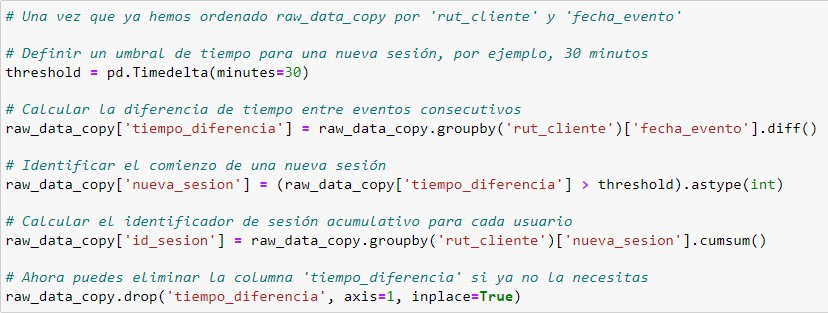
\includegraphics[width=\textwidth]{img/Código identificación sesiones.jpg}        
    \end{minipage}

    \begin{minipage}[t]{0.9\textwidth}
        Fuente: Elaboración propia.
    \end{minipage}
\end{figure}

Este método nos permitió estructurar el conjunto de datos de manera que refleja con precisión los períodos de interacción activa de los usuarios con el sistema, proporcionando una base sólida para el análisis y la modelación predictiva de su comportamiento futuro.

\subsection{Codificación de Categorías}

En el aprendizaje automático, es común encontrarse con datos categóricos, es decir, información que no está representada numéricamente, como los nombres de los métodos y canales en nuestro conjunto de datos. Para que estos datos puedan ser procesados por un modelo de clasificación, es necesario convertir estas categorías textuales en un formato numérico que el modelo pueda entender y manejar eficientemente. Este proceso se conoce como codificación de categorías y se llevó a cabo de la siguiente manera:

\subsubsection{Mapeo de Categorías a Números:}

\begin{itemize}
    \item Se crearon dos diccionarios: uno para \textbf{métodos} y otro para \textbf{canales}.
    \item Cada diccionario mapea una categoría textual única a un número entero único.
    \item Por ejemplo, el método \textbf{`login()`} podría mapearse al número 1, \textbf{`getAccounts()`} al número 2, y así sucesivamente.
\end{itemize}

\subsubsection{Aplicación de la Codificación:}

\begin{itemize}
    \item Utilizamos estos diccionarios para transformar todas las instancias de métodos y canales en nuestro DataFrame. Cada método y canal en el conjunto de datos fue reemplazado por su valor numérico correspondiente según los diccionarios de mapeo.
\end{itemize}

\subsubsection{Beneficios de la Codificación}

\begin{itemize}
    \item Esta transformación es crucial porque los modelos de aprendizaje automático funcionan mejor con variables numéricas, las cuales pueden ser sujetas a operaciones matemáticas y estadísticas durante el entrenamiento del modelo.
    \item Además, la codificación permite el uso de algoritmos de incrustación (embedding) que pueden capturar y representar más información sobre las categorías en dimensiones más ricas que un simple número entero.
\end{itemize}

El código para implementar la codificación de categorías es el siguiente:

\begin{figure}[H]
    \begin{minipage}[t]{0.9\textwidth}
        \caption{Código codificación de categorías}
        \label{codificación_categorias}        
    \end{minipage}

    \vspace{10pt}

    \begin{minipage}[b]{1\textwidth}
        \centering
        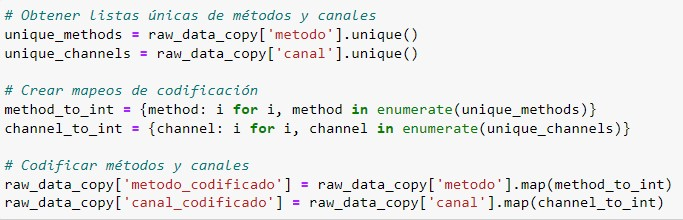
\includegraphics[width=\textwidth]{img/Código codificación categorias.jpg}        
    \end{minipage}

    \begin{minipage}[t]{0.9\textwidth}
        Fuente: Elaboración propia.
    \end{minipage}
\end{figure}

Esta etapa de codificación de categorías es un paso preparatorio esencial antes de alimentar los datos a nuestro modelo de clasificación secuencial. Permite que el modelo interprete adecuadamente los patrones en los métodos y canales como parte de la secuencia de acciones de un usuario y mejora la capacidad del modelo para hacer predicciones significativas sobre la próxima acción que el usuario podría tomar.

\subsection{Construcción de Secuencias}

La construcción de secuencias es un paso crucial en la preparación de datos para el modelado de series temporales o secuenciales, como es el caso de nuestro modelo de clasificación. Este proceso implica organizar los datos de tal manera que reflejen las secuencias naturales de interacciones de los usuarios. Veamos cómo se llevó a cabo:

\subsubsection{Agrupación de Eventos en Secuencias:}

\begin{itemize}
    \item Tras la codificación de los métodos y canales, cada acción del usuario está representada por un par de números codificados. El siguiente paso es agrupar estas acciones codificadas en secuencias que representan la trayectoria completa de la interacción del usuario dentro de una sesión.
    \item Cada secuencia se compone de pares de métodos y canales codificados y se crea para cada usuario y cada sesión identificada previamente. Esto se logra agrupando los datos por usuario y sesión y luego listando las acciones codificadas en orden cronológico.
\end{itemize}

\subsubsection{Preparación para el Modelo de Red Neuronal:}

\begin{itemize}
    \item Estas secuencias de números son lo que alimentará a la red neuronal. En el contexto de una LSTM o cualquier red neuronal recurrente (RNN), la secuencia permite al modelo reconocer patrones temporales y dependencias entre eventos consecutivos.
\end{itemize}

\subsubsection{Estructura de Datos de Secuencias:}

\begin{itemize}
    \item En términos de estructura de datos, las secuencias se manejan típicamente como listas de listas (o arrays de arrays) donde cada sublista representa una secuencia completa de un usuario.
\end{itemize}

El código para la construcción de secuencias es el siguiente:

\begin{figure}[H]
    \begin{minipage}[t]{0.9\textwidth}
        \caption{Código construcción de secuencias}
        \label{construcción_secuencias}        
    \end{minipage}

    \vspace{10pt}

    \begin{minipage}[b]{1\textwidth}
        \centering
        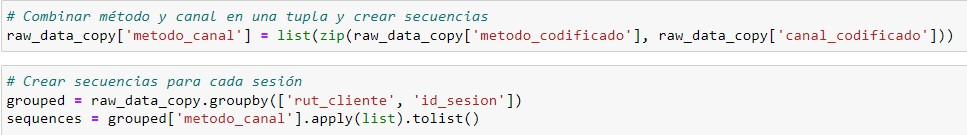
\includegraphics[width=\textwidth]{img/Código construcción de secuencias.jpg}        
    \end{minipage}

    \begin{minipage}[t]{0.9\textwidth}
        Fuente: Elaboración propia.
    \end{minipage}
\end{figure}

\subsubsection{Significado para el Modelado Predictivo:}

\begin{itemize}
    \item Estas secuencias son fundamentales para el modelado predictivo, ya que proporcionan el contexto completo necesario para que el modelo haga predicciones informadas. Por ejemplo, la secuencia de acciones anteriores de un usuario puede sugerir que la siguiente acción más probable podría ser \textquotedblright cerrar sesión\textquotedblright después de una serie de consultas de información.
\end{itemize}

\subsubsection{Alineación con Objetivos de Predicción:}

\begin{itemize}
    \item Además, las secuencias están alineadas con las etiquetas que se generaron en el paso de etiquetado, donde cada acción excepto la última en una secuencia tiene una etiqueta correspondiente que indica la acción siguiente. Esto permite entrenar al modelo en la tarea de predecir la siguiente acción basándose en la secuencia de acciones anteriores.
\end{itemize}

La construcción de secuencias, por lo tanto, transforma un conjunto de eventos individuales en una serie de caminos estructurados que reflejan el comportamiento y las decisiones del usuario, lo que es esencial para entrenar un modelo que pueda anticipar las siguientes acciones en la ruta del usuario

\subsection{División de Datos}
La partición de los datos en conjuntos específicos para el entrenamiento y la prueba constituye un aspecto crítico en el proceso de desarrollo de modelos de aprendizaje automático. Este paso es crucial para determinar la capacidad del modelo de generalizar a datos no observados previamente. En otras palabras, es fundamental para evaluar la habilidad del modelo para realizar predicciones precisas y fiables en nuevas entradas que no formaron parte del conjunto de datos de entrenamiento. A continuación, se detalla la metodología empleada para efectuar esta división de datos:

\subsubsection{Separación en Conjuntos de Entrenamiento y Prueba:}
El conjunto de datos completo se segmenta en dos partes principales: una sección destinada al entrenamiento del modelo, denominada el conjunto de entrenamiento, y otra sección utilizada para evaluar su rendimiento, conocida como el conjunto de prueba. Una práctica comúnmente aceptada en el campo del aprendizaje automático es asignar aproximadamente el 70-80\% del total de los datos para el entrenamiento y el 20-30\% restante para las pruebas. Esta proporción se elige para asegurar que el modelo tenga suficientes datos para aprender de manera efectiva, mientras se retiene una cantidad adecuada de datos no vistos para una evaluación fiable y representativa de su rendimiento.

\subsubsection{Aleatorización y Estratificación:}
Es imperativo que la división de los datos se realice de manera aleatoria para prevenir cualquier sesgo en la selección de estos. Este enfoque aleatorio asegura una representación equitativa y no sesgada de los datos en los conjuntos de entrenamiento y prueba. Adicionalmente, en situaciones donde el conjunto de datos es amplio y exhibe una diversidad considerable, resulta beneficioso implementar una técnica conocida como estratificación. La estratificación tiene como objetivo garantizar que la proporción de las distintas clases o categorías de respuesta se mantenga constante tanto en el conjunto de entrenamiento como en el de prueba. Este método es crucial para preservar la distribución representativa de las clases a lo largo de los conjuntos de datos, lo cual es vital para asegurar la validez y confiabilidad de la evaluación del modelo.

\subsubsection{Importancia para la Validación del Modelo:}
La división del conjunto de datos en distintas porciones para entrenamiento y prueba es una estrategia crucial para validar la eficacia del modelo en escenarios realistas. El propósito de esta separación es evaluar si el modelo es capaz de funcionar adecuadamente en condiciones que simulan el entorno real. En este contexto, el conjunto de prueba desempeña un papel vital, actuando como un sustituto de datos nuevos y no vistos en el mundo real. Al no haber sido expuesto a estos datos durante la fase de entrenamiento, el modelo se somete a una prueba rigurosa de su capacidad de generalización y robustez, lo cual es indispensable para determinar su aplicabilidad y fiabilidad práctica.

A continuación se presenta el fragmento de código implementado para la división del conjunto de datos. Este código es esencial para separar los datos en diferentes conjuntos, lo que permite una evaluación más precisa y objetiva del modelo:

\begin{figure}[H]
    \begin{minipage}[t]{0.9\textwidth}
        \caption{Código dividir el conjunto}
        \label{dividir_conjunto}        
    \end{minipage}

    \vspace{10pt}

    \begin{minipage}[b]{1\textwidth}
        \centering
        \includegraphics[width=\textwidth]{img/Código dividir el conjunto de entrenamiento.jpg}        
    \end{minipage}

    \begin{minipage}[t]{0.9\textwidth}
        Fuente: Elaboración propia.
    \end{minipage}
\end{figure}

\subsubsection{Protección Contra el Sobreajuste:}
En el proceso de entrenamiento de modelos de aprendizaje automático, se debe estar consciente del riesgo inherente de sobreajuste. Este fenómeno ocurre cuando el modelo se adapta excesivamente a los datos de entrenamiento, llegando a aprender y reproducir no solo las características subyacentes sino también el ruido y las particularidades idiosincrásicas de ese conjunto de datos. Para detectar y mitigar el sobreajuste, la división de los datos en conjuntos distintos para el entrenamiento y la validación/test es una práctica esencial. Esta estrategia permite evaluar el rendimiento del modelo en datos no vistos durante el entrenamiento, proporcionando así una medida más objetiva y fiable de su capacidad de generalización y su rendimiento real.

\subsubsection{Retroalimentación para la Iteración del Modelo:}
Los resultados obtenidos del conjunto de prueba son cruciales, ya que proporcionan información valiosa para el proceso iterativo de refinamiento y mejora del modelo. Un aspecto particularmente importante a observar es la comparación del rendimiento del modelo en el conjunto de prueba frente a su desempeño en el conjunto de entrenamiento. Una discrepancia notable, donde el modelo muestra un rendimiento significativamente inferior en el conjunto de prueba, sirve como un indicador claro de sobreajuste. Esta situación implica que, aunque el modelo ha aprendido eficientemente los patrones específicos de los datos de entrenamiento, no logra generalizar bien a nuevos datos, lo cual es un aspecto crítico en la evaluación de su aplicabilidad práctica.


\subsection{Construcción del Modelo}
La fase de construcción del modelo representa un momento crítico en el proceso de aprendizaje automático, en el cual se establece la arquitectura que el modelo empleará para aprender de los datos. En nuestro proyecto, hemos seleccionado un enfoque basado en un modelo de clasificación secuencial que emplea redes neuronales. Más específicamente, se ha implementado una Red Neuronal Recurrente (RNN) con unidades de Long Short-Term Memory (LSTM). Esta elección se basa en la habilidad de las RNN con LSTM para manejar eficientemente secuencias de datos, una característica esencial para nuestro objetivo de clasificación. A continuación, presentamos una descripción detallada de la estructura y configuración de este modelo:

\subsubsection{Selección de la Arquitectura:} 
La decisión de implementar una Red Neuronal Recurrente (RNN) con unidades de Long Short-Term Memory (LSTM) se fundamentó en su comprobada eficacia para el procesamiento de datos secuenciales. Las unidades LSTM son particularmente destacadas por su capacidad para aprender y retener dependencias de largo plazo presentes en los datos. Esta característica las hace extraordinariamente adecuadas para tareas que requieren una comprensión profunda del contexto secuencial, como es el caso de la predicción de la próxima acción de un usuario basándose en su historial de acciones previas. La habilidad de las LSTM para capturar estas dependencias temporales complejas y mantener información relevante a lo largo de secuencias extensas es un factor clave para el éxito en este tipo de aplicaciones de modelado predictivo.

\subsubsection{Capa de Incrustación (Embedding):} 
El modelo inicia su arquitectura con una capa de incrustación. La función principal de esta capa es convertir los índices correspondientes a métodos y canales, previamente codificados, en vectores densos de características. Esta transformación es crucial, ya que dota al modelo de la capacidad para interpretar de manera efectiva las entradas categóricas, facilitando la captura y el análisis de relaciones más complejas entre dichas entradas. La capa de incrustación juega un papel fundamental en el procesamiento de datos categóricos, mejorando significativamente la habilidad del modelo para discernir y aprender patrones y correlaciones subyacentes en los datos.

\subsubsection{Capas LSTM:} 
Subsiguiente a la capa de incrustación, se incorporaron una o varias capas de tipo Long Short-Term Memory (LSTM). Estas capas son especialmente adecuadas para el procesamiento de datos secuenciales, ya que están diseñadas para capturar dependencias a largo plazo y mantener un estado interno. Este estado interno actúa como un repositorio de información que refleja el contexto acumulado hasta el punto actual en la secuencia. La capacidad de las capas LSTM para recordar información a lo largo de secuencias extensas las hace particularmente valiosas en tareas donde el contexto y la secuencialidad de los datos son factores críticos para la precisión y eficacia del modelo.

\subsubsection{Capa Densa de Salida:} 
La configuración de la última capa de nuestro modelo consiste en una capa densa, diseñada con una unidad de salida para cada clase potencial, correspondiente en este contexto a cada acción posible siguiente. Esta capa crucial emplea la función de activación \textit{softmax}, que es esencial para convertir las salidas de la red en una distribución de probabilidad sobre las clases de acciones posibles. La aplicación de la función \textit{softmax} facilita que el modelo genere predicciones probabilísticas, asignando a cada clase potencial una probabilidad que refleja la confianza del modelo en esa acción específica como la acción siguiente más probable. Esta capacidad de producir una distribución de probabilidad es fundamental para el proceso de toma de decisiones y la interpretación de resultados en tareas de clasificación multiclase.
\begin{figure}[H]
    \begin{minipage}[t]{0.9\textwidth}
        \caption{Construccion del modelo de clasificación}
        \label{parquitectura_clasificación}        
    \end{minipage}

    \vspace{10pt}

    \begin{minipage}[b]{1\textwidth}
        \centering
        \includegraphics[width=\textwidth]{img/Arquitectura modelo clasificación.jpg}        
    \end{minipage}

    \begin{minipage}[t]{0.9\textwidth}
        Fuente: Elaboración propia.
    \end{minipage}
\end{figure}

\subsection{Regularización y Compilación}
En la fase actual del desarrollo de nuestro modelo, hemos centrado nuestra atención en dos componentes fundamentales: la regularización, con el propósito de evitar el sobreajuste, y la compilación, que establece los parámetros de cómo el modelo aprende y se optimiza durante el entrenamiento. A continuación, presentamos una descripción detallada de las estrategias y metodologías adoptadas para abordar eficientemente estos elementos esenciales:

\subsubsection{Regularización:} 
\begin{itemize}
    \item \textbf{Uso de Dropout:} Con el objetivo de mitigar el riesgo de sobreajuste, se integraron capas de Dropout en la arquitectura de nuestro modelo. El Dropout, una técnica de regularización bien establecida, funciona desactivando aleatoriamente un porcentaje determinado de neuronas durante cada iteración del proceso de entrenamiento. Esta estrategia impide que el modelo se vuelva excesivamente dependiente de cualquier conjunto específico de características o caminos neuronales, promoviendo así el aprendizaje de múltiples caminos redundantes y robustos para realizar predicciones. En la estructura de nuestro modelo, se incorporaron capas de Dropout sucesivamente a las capas LSTM y, en algunos casos, también después de las capas densas intermedias. El ratio de neuronas desactivadas se mantuvo comúnmente en un rango de 0.2 a 0.5, equilibrando efectivamente la regularización sin comprometer significativamente la capacidad de aprendizaje del modelo.
\end{itemize}

\subsubsection{Compilación del Modelo:} 
\begin{itemize}
    \item \textbf{Elección del Optimizador:} Para la compilación de nuestro modelo, se seleccionó el optimizador \textit{Adam} debido a su amplia aceptación y eficacia demostrada en una variedad de problemas en el campo del aprendizaje automático. Una de las características más destacadas de Adam es su capacidad para ajustar la tasa de aprendizaje de manera adaptativa a lo largo del proceso de entrenamiento. Este ajuste adaptativo facilita una optimización eficiente sin la necesidad de una intensiva afinación manual, haciéndolo un optimizador adecuado para una amplia gama de escenarios de aprendizaje automático. Su versatilidad y eficacia en la gestión de las tasas de aprendizaje lo convierten en una elección preferente para la compilación de modelos en diversos contextos de investigación y desarrollo.
    \item \textbf{Función de Pérdida:} En nuestro enfoque, se optó por utilizar la función de pérdida \textit{categorical\_crossentropy}, considerando la naturaleza del problema de clasificación multiclase con el que estamos trabajando. Esta función de pérdida es particularmente adecuada para situaciones donde las salidas del modelo son probabilidades. \textit{Categorical\_crossentropy} es eficaz para medir el rendimiento del modelo al comparar la distribución de probabilidad que el modelo predice con la distribución de probabilidad real, que está representada por las etiquetas de las clases. Esta comparación se centra en la precisión con la que el modelo es capaz de predecir la probabilidad correcta para cada clase en los datos, lo que es crucial en la clasificación multiclase.
    \item \textbf{Métricas de Evaluación:} Para el monitoreo del proceso de entrenamiento, se seleccionó la métrica de \textit{accuracy} (precisión). Esta métrica es una de las más intuitivas y comúnmente empleadas en el campo del aprendizaje automático, proporcionando una medida clara y directa del rendimiento del modelo. La precisión indica la proporción de predicciones correctas realizadas por el modelo en comparación con el número total de predicciones. Su amplia utilización se debe a su capacidad para ofrecer una comprensión rápida y efectiva de la eficacia general del modelo en la clasificación correcta de los datos.
\end{itemize}

\begin{figure}[H]
    \begin{minipage}[t]{0.9\textwidth}
        \caption{Construccion del compilador del modelo}
        \label{compilar_modelo}        
    \end{minipage}

    \vspace{10pt}

    \begin{minipage}[b]{1\textwidth}
        \centering
        \includegraphics[width=\textwidth]{img/Código compilar modelo.jpg}        
    \end{minipage}

    \begin{minipage}[t]{0.9\textwidth}
        Fuente: Elaboración propia.
    \end{minipage}
\end{figure}

\subsubsection{Balance entre Aprendizaje y Generalización} 
La implementación de la técnica de Dropout, en conjunto con una selección cuidadosa de la función de pérdida y el optimizador, tiene como objetivo fundamental establecer un balance óptimo en el rendimiento del modelo. Este balance se orienta hacia dos aspectos cruciales: por un lado, se busca que el modelo aprenda de manera eficiente a partir de los datos de entrenamiento, lo cual se manifiesta en la minimización de la pérdida. Por otro lado, se enfatiza la importancia de la capacidad del modelo para generalizar adecuadamente a nuevos conjuntos de datos, lo cual se refleja en una mayor precisión en el conjunto de prueba. La correcta armonización de estos elementos es esencial para garantizar que el modelo no solo se ajuste efectivamente a los datos con los que ha sido entrenado, sino que también mantenga un alto grado de precisión y relevancia al ser aplicado a datos no vistos anteriormente.

\subsubsection{Preparación para el Entrenamiento} 
Tras la compilación exitosa del modelo, este se encuentra preparado para entrar en la fase de entrenamiento. La compilación efectiva es un paso crucial, ya que garantiza que el proceso de entrenamiento se desarrolle de manera eficiente. Además, asegura que el modelo esté configurado adecuadamente para aprender patrones significativos de los datos, evitando así el riesgo de memorización excesiva. Este equilibrio es esencial para el rendimiento óptimo del modelo en aplicaciones del mundo real, donde la capacidad de generalización y adaptación a datos nuevos es fundamental.

\subsection{Entrenamiento del Modelo}
La fase de entrenamiento constituye el proceso esencial mediante el cual el modelo de clasificación secuencial adquiere conocimiento a partir de los datos. En esta etapa, el modelo realiza ajustes iterativos en sus parámetros internos con el objetivo primordial de minimizar el error en sus predicciones. Este proceso de optimización es fundamental para mejorar la precisión y la eficacia del modelo en la clasificación de datos. A continuación, se presenta una descripción detallada de cómo se implementó y ejecutó el entrenamiento del modelo:

\subsubsection{Alimentación de Datos al Modelo} 
El conjunto de datos de entrenamiento, que incluye tanto las secuencias de entrada (X\_train) como las etiquetas correspondientes (y\_train), se alimenta al modelo. El modelo aprende al ajustar sus pesos para predecir la etiqueta de cada secuencia de entrada lo más precisamente posible.

\subsubsection{Uso de Datos de Validación} 
De forma simultánea al proceso de entrenamiento, se emplea un conjunto de validación, designado como (X\_test, y\_test), para monitorear y evaluar el rendimiento del modelo. Esta práctica es fundamental, ya que proporciona información continua sobre la capacidad del modelo para generalizar a datos no previamente vistos. La utilización de este conjunto de validación es un componente esencial para garantizar que el modelo no está incurriendo en un sobreajuste con respecto a los datos de entrenamiento. Al evaluar cómo el modelo se desempeña con un conjunto de datos independiente, se puede obtener una perspectiva más objetiva y realista sobre su eficacia y potencial aplicabilidad en escenarios del mundo real.

\subsubsection{Configuración del Proceso de Entrenamiento} 
El proceso de entrenamiento del modelo se estructura en un número específico de iteraciones, denominadas épocas. Durante cada una de estas épocas, el modelo procesa de manera completa el conjunto de datos de entrenamiento. Esta metodología permite que el modelo refine iterativamente sus parámetros internos a través de la exposición repetida a todo el conjunto de entrenamiento. Este enfoque secuencial asegura una evolución sistemática y progresiva de la capacidad del modelo para aprender y adaptarse a las características inherentes a los datos.

\subsubsection{Monitoreo con EarlyStopping} 
Con el objetivo de prevenir el fenómeno de sobreajuste durante el entrenamiento del modelo, se ha implementado una técnica conocida como EarlyStopping. Este método consiste en monitorear de manera continua la pérdida observada en el conjunto de validación. El entrenamiento se interrumpe automáticamente cuando no se percibe una mejora en esta métrica de pérdida tras un número predefinido de épocas. Esta estrategia es crucial para asegurar que el modelo no se ajuste excesivamente a los datos de entrenamiento, perdiendo así su capacidad de generalización.

Adicionalmente, se ha activado la opción restore\_best\_weights dentro de la funcionalidad de EarlyStopping. Esto implica que, al finalizar el entrenamiento prematuro, el modelo restaura automáticamente los pesos correspondientes a la época en la que se logró la menor pérdida de validación. Este enfoque garantiza que el modelo retenido es el que ha demostrado el mejor rendimiento en términos de generalización, según lo medido por la pérdida en el conjunto de validación.


\subsubsection{Evaluación del Rendimiento} 
Durante la fase de entrenamiento del modelo, se lleva a cabo un monitoreo constante de las métricas de precisión y pérdida, tanto en los conjuntos de entrenamiento como en los de validación. Estas métricas son fundamentales para evaluar el rendimiento del modelo, ya que proporcionan información crítica sobre su capacidad para aprender de los datos y generalizar a nuevos conjuntos de datos. El análisis continuo de la precisión y la pérdida es esencial para identificar la eficacia con la que el modelo se está ajustando a los datos. Este proceso ayuda a detectar problemas potenciales, como el sobreajuste o el subajuste, y permite realizar ajustes oportunos en los parámetros del modelo o en la estrategia de entrenamiento para optimizar su rendimiento.

\begin{figure}[H]
    \begin{minipage}[t]{0.9\textwidth}
        \caption{Código para entrenar el modelo}
        \label{entrenar_modelo}        
    \end{minipage}

    \vspace{10pt}

    \begin{minipage}[b]{1\textwidth}
        \centering
        \includegraphics[width=\textwidth]{img/Código entrenar el modelo.jpg}        
    \end{minipage}

    \begin{minipage}[t]{0.9\textwidth}
        Fuente: Elaboración propia.
    \end{minipage}
\end{figure}


\subsection{Resultados del entrenamiento del modelo}

Una vez finalizado el proceso de entrenamiento del modelo, procedimos a evaluar su rendimiento. Esta evaluación se basó en el análisis detallado de las métricas de pérdida y precisión, tanto en el conjunto de entrenamiento como en el conjunto de validación. Este enfoque nos permite comprender de manera integral cómo el modelo se comporta en diferentes conjuntos de datos, destacando tanto su eficacia en el aprendizaje como su capacidad de generalización a nuevos datos. La comparación de estas métricas entre los conjuntos de entrenamiento y validación es fundamental para identificar posibles problemas de sobreajuste o subajuste, y para asegurar la robustez y fiabilidad del modelo en aplicaciones prácticas.
\subsubsection{\textbf{Análisis de la Pérdida}} 
El análisis de los gráficos revela que tanto la pérdida de entrenamiento (Loss) como la pérdida de validación (Val\_Loss) experimentan una disminución significativa durante las etapas iniciales del proceso de entrenamiento. Este comportamiento indica que el modelo está aprendiendo de manera efectiva a partir de los datos proporcionados. Con el progreso de las épocas de entrenamiento, se observa que ambas curvas de pérdida tienden a estabilizarse y a converger. Dicha convergencia es indicativa de que el modelo ha alcanzado un estado en el cual puede realizar predicciones consistentes y confiables.

La proximidad en la trayectoria de las curvas de pérdida de entrenamiento y de validación es un indicador clave de que el modelo no está incurriendo en un sobreajuste. Esto se evidencia por el hecho de que la pérdida de validación no muestra un incremento o divergencia significativa respecto a la pérdida de entrenamiento, lo cual sería una señal clara de sobreajuste. Por tanto, estos resultados sugieren que el modelo ha logrado un equilibrio adecuado en su capacidad de generalización a partir de los datos de entrenamiento.

\subsubsection{\textbf{Análisis de la Precisión}} 

En relación con la métrica de precisión, se observa que tanto la precisión durante el entrenamiento (Accuracy) como la precisión durante la validación (Val\_Accuracy) muestran un incremento significativo en las fases iniciales, seguido de una fase de estabilización donde ambas métricas se mantienen en valores cercanos entre sí. Este patrón de comportamiento es indicativo de un alto grado de exactitud en las predicciones generadas por el modelo. Además, la proximidad entre la precisión de entrenamiento y la de validación sugiere que el modelo posee una buena capacidad de generalización frente a nuevos conjuntos de datos.

Esta tendencia en las métricas de precisión es un factor alentador, ya que implica que el modelo no solo es eficaz en el reconocimiento de patrones en los datos de entrenamiento, sino que también mantiene un rendimiento consistente cuando se expone a datos no vistos durante la fase de entrenamiento. Esta característica es esencial para la aplicabilidad práctica del modelo en entornos reales, donde la capacidad de generalizar a partir de datos nuevos y variados es crucial.

\begin{figure}[H]
    \begin{minipage}[t]{0.9\textwidth}
        \caption{Gráficos de análisis del modelo de clasificación}
        \label{gráfico_clasificación}        
    \end{minipage}

    \vspace{10pt}

    \begin{minipage}[b]{1\textwidth}
        \centering
        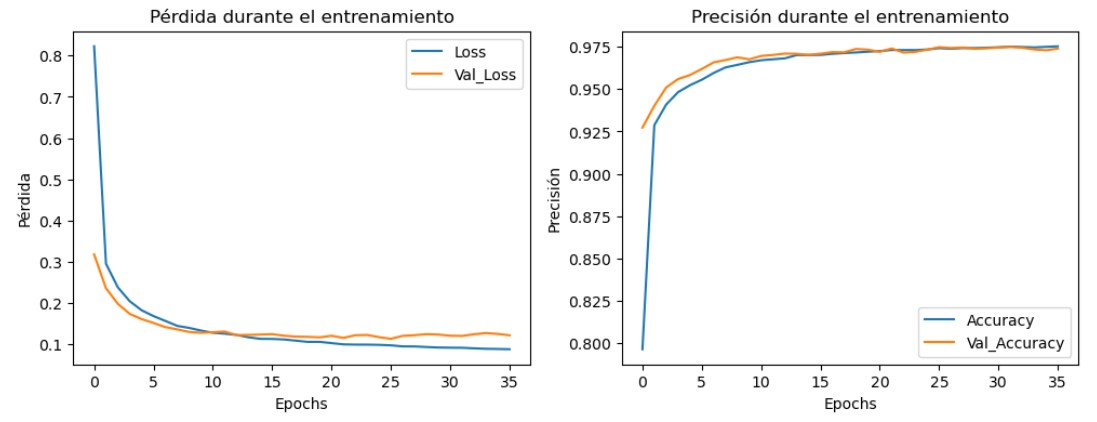
\includegraphics[width=\textwidth]{img/Gráfico modelo clasificación.jpg}        
    \end{minipage}

    \begin{minipage}[t]{0.9\textwidth}
        Fuente: Elaboración propia.
    \end{minipage}
\end{figure}

\subsection{Predicción del modelo}

En la aplicación de nuestro modelo de clasificación secuencial para la generación de predicciones, se procesa una secuencia de acciones previas ejecutadas por un usuario. El modelo utiliza este historial para inferir cuál podría ser la siguiente acción del usuario. Un aspecto distintivo de este modelo es su capacidad no solo para identificar la acción subsiguiente más probable, sino también para cuantificar la confianza en dicha predicción, expresándola en términos de probabilidad.

Por ejemplo, consideremos un caso donde el historial de un usuario indica que está en proceso de recolección de información. Si el modelo anticipa que la acción siguiente será \texttt{getDetails()}, esta predicción se acompaña de una probabilidad asignada, por ejemplo, del 95\%. Tal porcentaje refleja la confianza del modelo en que \texttt{getDetails()} será la próxima acción del usuario. Esta métrica de confianza es fundamental para interpretar no solo las expectativas del modelo sobre eventos futuros, sino también el nivel de certeza asociado a estas expectativas.

En un escenario diferente, si un usuario ha estado interactuando con su cuenta y el modelo pronostica que la acción siguiente será \texttt{getSSContributionsCertificate()}, esta predicción puede presentar una probabilidad del 78.76\%. Este valor sugiere que, aunque el modelo se inclina por \texttt{getSSContributionsCertificate} como la acción probable, existe una notable incertidumbre, posiblemente atribuible a la variabilidad en el comportamiento del usuario o a patrones ambiguos en sus acciones anteriores.

Estos ejemplos demuestran cómo el modelo va más allá de la toma de decisiones binarias, proporcionando un marco cuantitativo que resulta invaluable para la toma de decisiones basada en datos. Este enfoque permite a los sistemas automatizados o a los operadores humanos comprender con mayor profundidad y responder de manera más efectiva a las predicciones generadas por el modelo.
\subsection{Métricas de predicción aplicadas}

Explicaremos a continuación las métricas utilizadas para evaluar el rendimiento del modelo de clasificación, detallando también los resultados obtenidos y su interpretación:

\subsubsection{Precisión (Precision)}
La precisión constituye una métrica crítica en la evaluación de modelos de clasificación. Esta métrica proporciona una estimación de la fiabilidad de las predicciones positivas generadas por el modelo. En términos más concretos, la precisión representa el porcentaje de instancias clasificadas correctamente como positivas por el modelo, en relación con el total de instancias que el modelo ha identificado como positivas, particularmente en escenarios de clasificación multiclase.

Al referirse a una precisión del 57.94\% (o 0.5794 en formato decimal), se está indicando que, bajo las condiciones actuales de modelado, existe una probabilidad del 57.94\% de que una instancia clasificada por el modelo en una categoría específica sea una clasificación acertada. Esta interpretación de la precisión es crucial para comprender la eficacia del modelo en la identificación correcta de las categorías relevantes.

\subsubsection{Recall (Sensibilidad o Tasa de Verdaderos Positivos)}
El \textit{recall} es una medida que indica qué proporción de instancias realmente positivas han sido identificadas correctamente por el modelo. Es decir, del total de instancias que verdaderamente pertenecen a una clase, el \textit{recall} muestra qué porcentaje ha sido reconocido de forma acertada por el modelo.

Con un \textit{recall} de 0.5487 (o 54.87\%), esto sugiere que el modelo logra identificar correctamente el 54.87\% de todas las instancias positivas presentes en el conjunto de datos.

\subsubsection{Puntuación F1}

La puntuación F1 constituye una métrica integral en la evaluación del rendimiento de un modelo de clasificación. Esta métrica es particularmente relevante cuando se busca un equilibrio entre la precisión (precision) y el recall, siendo especialmente útil en contextos donde existe una distribución desigual de clases. Dicho desequilibrio se presenta cuando una clase es significativamente más frecuente que otra.

La puntuación F1 se define como la media armónica de la precisión y el recall. Esta media tiende a favorecer los valores menores dentro del conjunto, lo que implica que un rendimiento alto tanto en precisión como en recall es esencial para alcanzar una puntuación F1 elevada. La puntuación F1 varía entre 0 y 1, donde 1 representa la perfección y 0 la peor puntuación posible.

En el caso de nuestro modelo, con una puntuación F1 de 0.5366 (o 53.66\%), se refleja un equilibrio moderado entre la precisión y el recall. Una puntuación de 53.66\% sugiere un desempeño intermedio, indicando que el modelo no sobresale en ninguna de las dos métricas de manera excepcional, pero tampoco presenta deficiencias significativas. Sin embargo, se preferiría una puntuación F1 más alta, lo que indicaría una mayor armonía y efectividad en el equilibrio entre precisión y recall.

\subsection{Conclusión del Modelo de Predicción Secuencial}

El modelo de predicción de secuencias se ha desarrollado con el propósito de anticipar futuras acciones de usuarios basándose en patrones de comportamiento históricos. Aunque el modelo demuestra una capacidad moderada en la clasificación y predicción de estas acciones, evidenciado por una precisión del 57.94\% y un recall del 54.87\%, los resultados sugieren que existe un margen considerable para mejorar tanto su precisión como su fiabilidad.

La puntuación F1 de 53.66\% refleja un equilibrio entre la precisión y el recall, pero también destaca la necesidad de optimizar el modelo para mejorar su rendimiento predictivo. Esto podría realizarse a través de la refinación de la arquitectura del modelo, la implementación de ajustes en la regularización o la utilización de un conjunto de datos más extenso o representativo.

A pesar de que el modelo actual constituye un punto de partida robusto para la predicción de comportamientos futuros basándose en datos históricos, es claro que para aplicaciones que requieren alta precisión o son críticas, se hace imprescindible una optimización y evaluación adicional. Este proceso de análisis y mejora continua es crucial, particularmente en contextos donde los errores en la predicción podrían tener implicaciones significativas.

Por lo tanto, aunque el modelo actual no alcanza aún los estándares requeridos para una predicción altamente precisa y confiable, representa un avance significativo hacia el entendimiento y la anticipación del comportamiento del usuario. La estrategia a futuro se centrará en la mejora y ajuste del modelo existente, así como en la exploración de nuevas técnicas y metodologías que se alineen más efectivamente con los objetivos de predicción del comportamiento.